\documentclass[a4paper, 12pt]{article}

\usepackage{graphicx}
\usepackage{xcolor}
\usepackage{mdframed}
\usepackage { amsmath , amssymb , amsthm }
\usepackage[T2A]{fontenc}
\usepackage[utf8]{inputenc}
\usepackage[english,russian]{babel}

\graphicspath{{img/}}
\DeclareGraphicsExtensions{.pdf,.png,.jpg}


\title{Д.М. Домашнее задание}
\author{Осипенко Данил, 595гр.}
\date{\today}

\begin{document}
\sffamily
\maketitle

\section*{16}
$ A = \{0,2,3,7,8\}, B = \{1,3,6,7,9\}, C = \{0,1,4,7,8,9\}, I = \{0,1,2,\ldots,9\} $
\[
    P = \overline{B}\cap_1\overline{C}\cup_2 A\cap_3 C \cup_4 A \cap_5 \overline{B}     
\]
$ \overline{B} = \{2,4,5,8\},\overline{C} = \{2,3,5,6\} $\\
$ 1: \{2,5\};2:\{0,2,3,5,7,8\};3:\{0,7,8\};4: \{0,2,3,7,8\};5:\{2,8\} $
\[
       \underline{P = \{2,8\}}
\]
\section*{36}
$ A = \{0,3,4,9\},C = \{0,1,2,4,7,8,9\}, B = \{1,3,4,7\}, I = \{0,1,2,\ldots,9\}$
\[
       P = ((((((A\cap C)\cup A) \cap \overline{B}) \cup \overline{B}) \cap C) \cup 
       \overline{A}) \cap \overline{B}
\]
$ 1: (A\cap C)\cup A = A ;\\
2:(A \cap \overline{B}) \cup \overline{B} = \overline{B},\\
3:((\overline{B} \cap C) \cup \overline{A}) = (\overline{B} \cup \overline{A})\cap (C \cup \overline{A})\\
4:((\overline{B} \cup \overline{A})\cap (C \cup \overline{A}))\cap \overline{B} = \overline{B} \cap (\overline{B}\cap(C\cup \overline{A}))\\
5:\overline{P} = \overline{\overline{B}\cap(C\cup \overline{A})} = B \cup (\overline{C} \cap A)\\
\overline{C} = \{3,5,6\}$
\[
       \underline{P = \{1,3,4,7\}}
\]
\newpage
\section*{56}
\[
       (((((B\cap \overline{C})\cap \overline{D}) \cup \overline{B}) \cap C) \cup \overline{A}) \cap B
\]
$1: (B\cap \overline{C}) = \emptyset\\
2: \emptyset \cap \overline{D} = \emptyset\\
3: \emptyset \cup \overline{B} = \overline{B}\\
4: (\overline{B} \cap C) = C \setminus B\\
5: (C \setminus B)\cup \overline{A} = C\setminus A\\
6: (C\setminus A) \cap B = B \setminus A $
\[
       \underline{B \setminus A}
\]
\section*{76}
\[
       \overline{P} + \overline{P}Q + \overline{P}Q\overline{R} + \overline{P}T
\]
\[
       \underline{\overline{P}(1 + Q + Q\overline{R} + T) = \overline{P}}
\]
\section*{96}
\[
    ABE + \overline{A}\overline{B}\overline{E} + B\overline{C}\overline{E}       
\]
\[
    \overline{ABE + \overline{A}\overline{B}\overline{E} + B\overline{C}\overline{E}} = \underline{(\overline{A}+\overline{B}+\overline{E})(A + B + C)(\overline{B} + C + E)}
\]

\section*{136}
\[
       f = AB + \overline{A} \overline{B}
\]
\[
       \underline{f(2,11)}
\]
\section*{156}
\[
       (2,3,4,8,13,14)
\]
\begin{center}
       \begin{tabular}{| c | c c c c | c|} 
       \hline
       n & A & B & C & D & F \\ 
       \hline
       2 & 0 & 0 & 1 & 0 & 1 \\ 
       \hline
       3 & 0 & 0 & 1 & 1 & 1 \\
       \hline
       4 & 0 & 1 & 0 & 0 & 1 \\
       \hline
       8 & 1 & 0 & 0 & 0 & 1 \\
       \hline
       13 & 1 & 1 & 0 & 1 & 1 \\
       \hline
       14 & 1 & 1 & 1 & 0 & 1 \\
       \hline
      \end{tabular}
\end{center}
\[
       f = \overline{AB}C\overline{D} + \overline{AB}CD + \overline{A}B\overline{CD} + A\overline{BCD} + AB\overline{C}D + ABC\overline{D} = \underline{1 + \overline{A} + A\overline{D}}
\]
\underline{2 с 13 $ (\overline{AB}C\overline{D} + AB\overline{C}D = 1)$, 3 с 4 $ (\overline{AB}CD + \overline{A}B\overline{CD} = \overline{A}(\overline{B}CD + B\overline{CD}) = \overline{A}) $
,}\\ \underline{8 c 14 $ (A\overline{BCD} + ABC\overline{D} = A\overline{D}) $}
\section*{336}
\[
       X + BC + \overline{A}C = C + \overline{A}B
\]
\begin{center}
       \begin{tabular}{| c | c c c | c | c  | c |} 
       \hline
       n & A & B & C & X & $ F_1 $ & $ F_2 $ \\ 
       \hline
       0 & 0 & 0 & 0 & 0 & 0 & 0\\ 
       \hline
       1 & 0 & 0 & 1 & 0 & 1 & 1\\ 
       \hline
       2 & 0 & 1 & 0 & 0 & 0 & 1 \\
       \hline
       3 & 0 & 1 & 1 & 0 & 1 & 1\\
       \hline
       4 & 1 & 0 & 0 & 0 & 0 & 0\\
       \hline
       5 & 1 & 0 & 1 & 0 & 0 & 1\\
       \hline
       6 & 1 & 1 & 0 & 0 & 0 & 0\\
       \hline
       7 & 1 & 1 & 1 & 0 & 1 & 1\\
       \hline
       8 & 0 & 0 & 1 & 1 & 1 & 1\\ 
       \hline
       9 & 0 & 1 & 0 & 1 & 1 & 1 \\
       \hline
       10 & 0 & 1 & 1 & 1 & 1 & 1\\
       \hline
       11 & 1 & 0 & 0 & 1 & 1 & 0\\
       \hline
       12 & 1 & 0 & 1 & 1 & 1 & 1\\
       \hline
       13 & 1 & 1 & 0 & 1 & 1 & 0\\
       \hline
       14 & 1 & 1 & 1 & 1 & 1 & 1\\
       \hline
       15 & 0 & 0 & 0 & 1 & 1 & 0\\ 
       \hline
       
      \end{tabular}
\end{center}
\[
       \underbrace{1 + C + \overline{A}BC}_X + BC + \overline{A}C = C + \overline{A}B
\]576
\section*{536}
\[
       9 \quad 5 \quad 8
\]
\[
       \underline{C^8_9 9^1 = 81} 
\]
\section*{556}
\[
       n^m * l = 7^3 * 4 = \underline{1372}
\]
\newpage
\section*{576}
\[
       \{\{1,2\},\{1,3\},\{1,8\},\{2,3\},\{2,4\},\{3,4\},\{3,5\},\{4,5\},\{4,5\},\{5,6\}
       ,\{6,7\},\{6,8\},\{7,8\}\}
\]
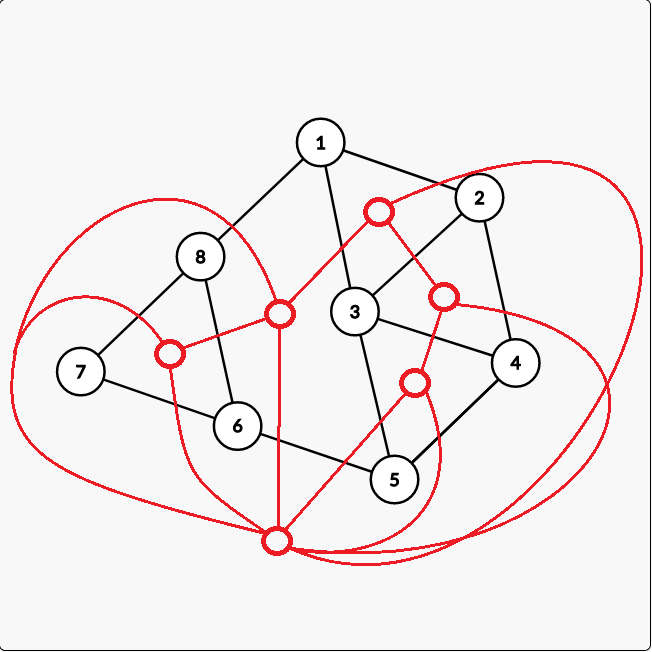
\includegraphics{576.png}\\
\underline{число вершин - 6; число ребер - 12; число граней - 8;}
\section*{596}
\[
       \{\{1,2\},\{1,4\},\{2,3\},\{2,4\},\{2,5\},\{3,4\},\{3,6\},\{4,5\},\{4,6\},\{5,6\},\}
\]
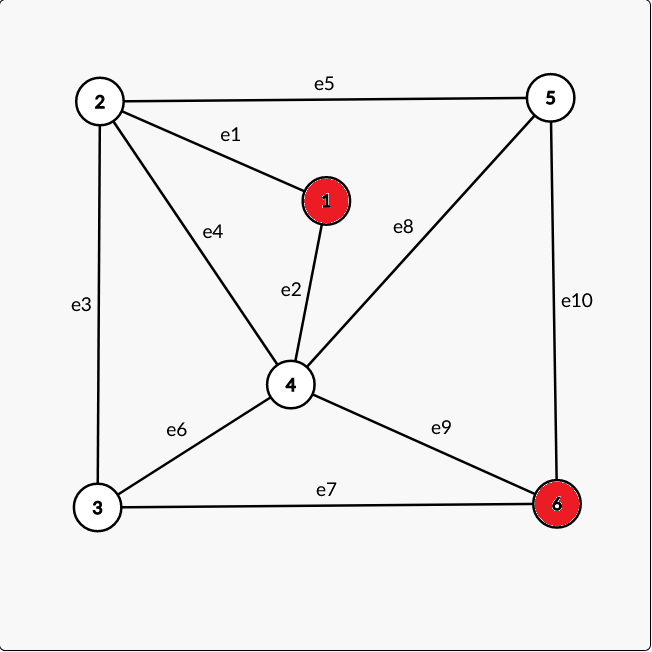
\includegraphics{596.png}\\
\begin{center}
    \begin{tabular}{l | l}
       1 e1 2 e3 3 e7 6 & 1 e1 2 e3 3 e6 4 e8 5 e10 6\\\hline
       1 e1 2 e3 3 e6 4 e9 6 & 1 e1 2 e4 4 e8 5 e10 6\\\hline
       1 e1 2 e4 4 e9 6 & 1 e1 2 e4 4 e6 3 e7 6\\\hline
       1 e1 2 e5 5 e10 6 & 1 e1 2 e5 5 e8 4 e6 3 e7 6\\\hline
       1 e1 2 e5 5 e8 4 e9 6 & 1 e2 4 e9 6\\\hline
       1 e2 4 e6 3 e7 6 & 1 e2 4 e6 3 e3 2 e5 5 e10 6\\\hline
       1 e2 4 e4 2 e3 3 e7 6 & 1 e2 4 e4 2 e5 5 e10 6\\\hline
       1 e2 4 e8 5 e10 6 & 1 e2 4 e8 5 e5 2 e3 3 e7 7.        
    \end{tabular}
\end{center}
\newpage
\section*{616}
\[
    K = (2,2,4,9,2,2,9,9)
\]
$ \{\{1,2\},\{2,3\},\{2,6\},\{2,7\},\{2,9\},\{4,5\},\{4,9\},\{8,9\}\{9,10\}\} $\\
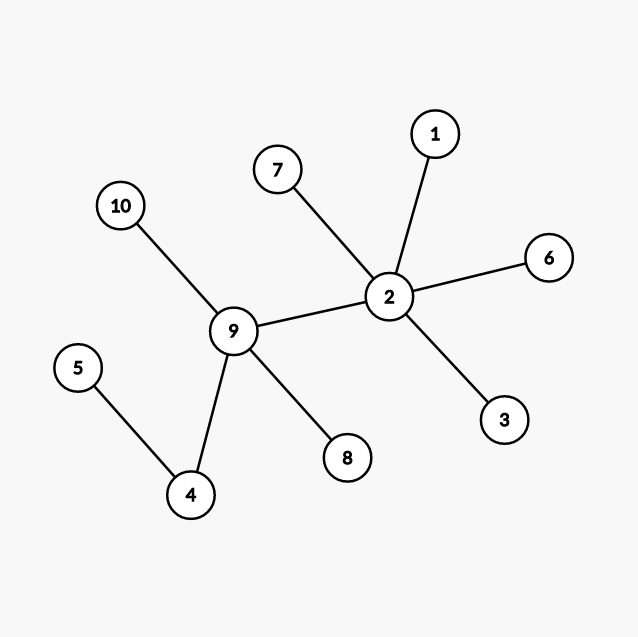
\includegraphics{616.png}\\





 




\end{document}